\chapter{Déroulement}\thispagestyle{fancy}

\paragraph{}
Cette chapitre explique les travaux principale pendant mon stage. Il se compose de trois sections. Tous d'abord, j'ai installé et configuré un environnement de développement afin de améliorer l'efficacité. Ensuit, le travaille principale est l'amélioration du framework KdoMotiv Médium. Dernièrement, c'est quelque projets lesquels j'ai réalisé par KdoMotiv.

\section[Configuration]{Configuration de l'environnement}

\subsection{Installer un serveur linux local}
\paragraph{}
Comme le problème j'ai expliqué dans le chapitre avant, ce n'est pas très pratique avec un serveur disant sans droits ou un serveur local avec système exploitation de windows.
Auparavant, quand les collègue de pôle web avait le problème sur quelque site, ils doivent communiquer directement chez notre pôle. En plus, il n'y a rien de trace ou histoire sur le problème. 
Par conséquent, j'ai choisi un ordinateur qui n'est utilisé plus comme un nouveau serveur local. 

Lorsque ubuntu est un système d'exploitation intuitif et sécurisé, idéal pour les ordinateurs de bureau, les serveurs, les netbooks et les ordinateurs portables. En plus, Ubuntu est libre, gratuit, et est composé de logiciels qui le sont également.

J'ai décidé d'installer ubuntu serveur 10.04(LTS\footnote{Long Term Support}) sur serveur local.

\subsubsection{Partition}
En fait, comme le serveur local n'est pas très puissant,il a juste 2G de RAM de ce PC.  il faut l'attribuer 2G de swap. La partition de disque est comme la table suivant.

\begin{table}[htbp]
\centering
\begin{tabular}{ll}
  \toprule
  Partition & G\\
  \midrule
	/ & 30 \\ 
	\hline 
	swap & 2 \\ 
	\hline 
	/var & 10 \\ 
	\hline 
	/tmp & 5 \\ 
	\hline 
	/home & reste \\
  \bottomrule
\end{tabular}
 \caption{\label{tab:Partition du serveur}Partition du serveur}
\end{table}

\subsubsection{Installation de l'environnement LAMP + PhpMyAdmin}
LAMP est un acronyme désignant un ensemble de logiciels libres permettant de construire des serveurs de sites web. L'acronyme original se réfère aux logiciels suivants :
\begin{itemize}
\item[•] Linux 
\item[•] Apache 
\item[•] MySQL 
\item[•] PHP 
\end{itemize}
Sur ce serveur local, on a aussi besoin de debuger le site php ou développer quelque fonctions de php sert à traiter les données locales. Il faut configurer un environnement plus proche ou similaire que l'environnement LAMP sur serveur distant. Pourquoi mettre un environnement plus similaire que celui sur serveur production? Au cas où si on va déployer ce que on a développer sur serveur local, mais ne fonctionne pas sur serveur de production. 

D'ailleurs, afin de contrôler le serveur plus facilement, j'ai aussi installé le OPENSSH. Après cette étap, je peux faire tous les opérations sur ma poste avec PuTTY\footnote{PuTTY est un émulateur de terminal doublé d'un client pour les protocoles SSH, Telnet, rlogin, et TCP brut.}

Mais, il y a encore de un peu de problème de ce serveur. Tous d'abord, comme c'est un PC dans réseau local, on n'a pas fixer l'adresse IP de cette machine. S'il a éprouvé la situation de coupure d'électricité de week-end, et le serveur a redémarré automatiquement, l'adresse IP de cette machine serait changé à cause de DHCP. C'est-à-dire chaque fois, on doit informer à les autre département du changement de l'adresse IP de serveur local.

Ce n'est pas pratique. La solution sera fixé l'adresse ip depuis la configuration du routeur.



\subsubsection{Installation de Ruby on Rails et RedMine}
Comme le problème lequel j'ai déjà expliqué dans le chapitre avant, ce n'est pas pratique de communiquer entre différent pôle  et suivre ou tracer des bugs de tous les projets. 

Par conséquent, j'ai trouver deux applications web candidats qui sert à la gestion de projet. Une est RedMine qui est programmé par Ruby, l'autre est Trac qui est programmé par python. Finalement, j'ai fixé d'utiliser RedMine dû à son plus agréable interface.  

Vu que RedMine est une web application sous framework Ruby on Rails. Il faut configurer la framework de ROR sur serveur local. 

Après l'installation et la configuration du ROR, la mise en place de Redmine est simple. Suivi les instructions depuis le site officiel de Redmine, c'est simple de mettre en œuvre. 

Ensuite, j'ai déposé tous les projets actuels de Data-Gest afin de gérer et tracer sur RedMine. On peut aussi apercevoir les anomalies, les évolution, les assistances de chaque projet.
\begin{figure}[hbtp]
\centering
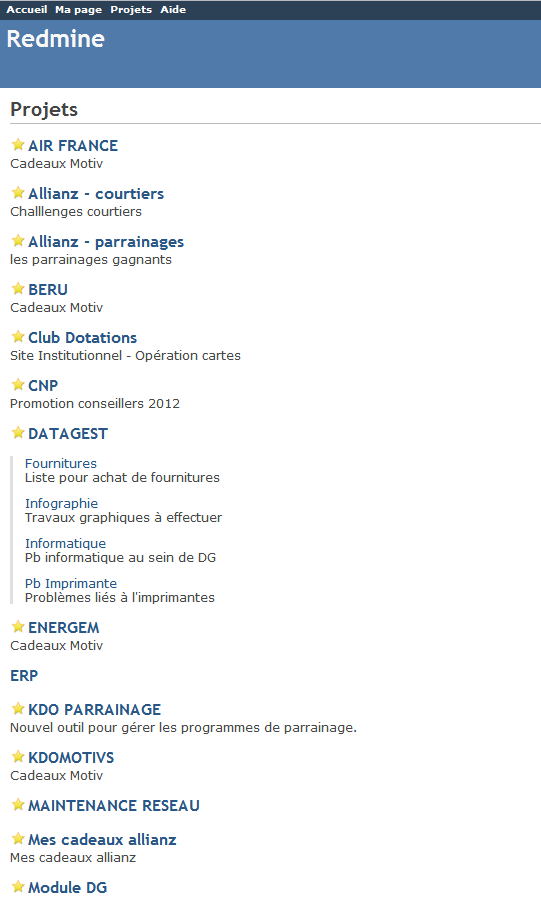
\includegraphics[width=10cm]{body/images/redmine-accueil.PNG}
\caption{Acceuil de Redmine}
\end{figure}



Cependant, quand j'ai essayé d'ajouter un ticket sur redmine à la fin du test, je n'ai reçu aucune  mail de notification lorsque le changement de ticket.

\subsubsection{Installation du serveur mail(Postfix) local}
Afin de fixer le problème que j'avais avant concernent le mails. J'ai installé le Postfix comme le serveur de messagerie électronique au remplacement du serveur \textbf{Sendmail}, vu qu'il est plus léger et plus stable. La configuration de Postfix en détail est dans annexe.

\subsubsection{Résume}
Étant donné que le serveur local peut juste être visité pas adresse IP, mais il y a plusieurs services sur ce serveur. Par conséquence, j'ai configuré les différent portes de Apache ou on peut y accéder pour utiliser le différent service. Par exemple, si on va accéder à PhpMyAdmin\footnote{Interface graphique pour gérer MySQL}, on peut juste ajout la porte correspondant après l'adresse IP.

\begin{table}[htbp]
\centering
\begin{tabular}{ll}
  \toprule
  Porte & Service\\
  \midrule
	80(Par défaut) & l'application RedMine \\ 	 
	8080 & CMS Drupal, développement de site par Drupal \\ 	 
	8888 & PhpMyAdmin, interface graphique pour la gestion Base de donnée \\ 	 
  \bottomrule
\end{tabular}
 \caption{Service de différents portes}
\end{table}

\subsection{Configuration un serveur SVN sur seveur distant}
\paragraph{}
Quand le serveur distant OHV est mise en œuvre, le SVN est déjà pré-installé sur le serveur dev, c'est-à-dire on peut contrôler lès version de projets que on a déjà développé. Mais on a pas bien communiqué avec l'administrateur réseaux d'OVH, et on n'a utilisé jamais depuis un an. Après le nouveaux chef de gestion de projet est arrivé, on l'a décidé de reprendre. 

Mais il semble que le SVN sur serveur dev distant est mal configuré, il y a juste un dépôt de subvention par défaut sur le serveur. En plus, on a pas de droit de le configuré soi-même. Par conséquence, on a demandé  à l'administrateur réseaux d'ovh de nous donner tous les droits d'en contrôler. 

\subsubsection{Fichier de conf}
Après on a gagné les droit de configuration dans le répertoire de SVN, on a créé un dépôt qui sert à notre premier projet lequel on voudrait contrôler la version en ligne de commande. Dans le répertoire "\textbf{conf}" de ce dépôt subvention, on peut ajouter les utilisateurs qui peuvent faire les action "commit" à ce dépôt  ou "check out" depuis ce dépôt. 
\begin{figure}[hbtp]
\centering
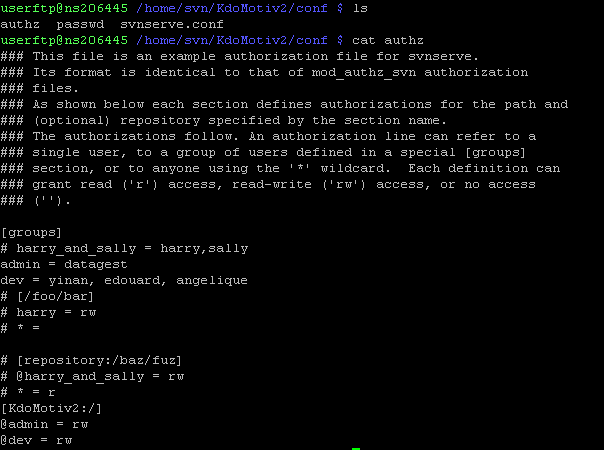
\includegraphics[width=10cm]{body/images/conf-svn.png}
\caption{fichier conf SVN}
\end{figure}


\subsubsection{Problème de permission de répertoire }
On a installé TortoiseSVN comme le logiciel de côté client.  Mais on a eu le problème de la permission de commit pendant le commit. En fait, le dépôt on a créé est dans le groupe de "user". Mais quand on fait un commit depuis côté client, c'est le utilisateur svn dans groupe svn qui le fait par défaut, il n'a pas de droit d'écrire et lire dans répertoire de dépôt.

On doit lancé a commande dans linux afin de changer l'utilisateur et le groupe d'une répertoire dans le dépôt. 

\begin{figure}[hbtp]
\centering
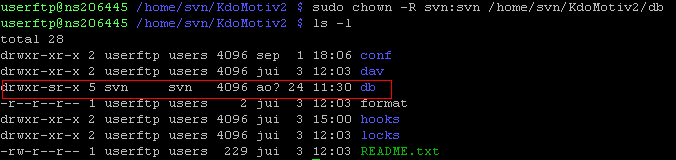
\includegraphics[width=10cm]{body/images/svn-problem-permission.png}
\caption{Changer groupe de répertoire}
\end{figure}

\subsubsection{WEBSVN}
WEBSVN est un interface graphique permettant de visualiser les versions des projets. Il est pointé vers le répertoire de dépôt de SVN.
\begin{figure}[hbtp]
\centering
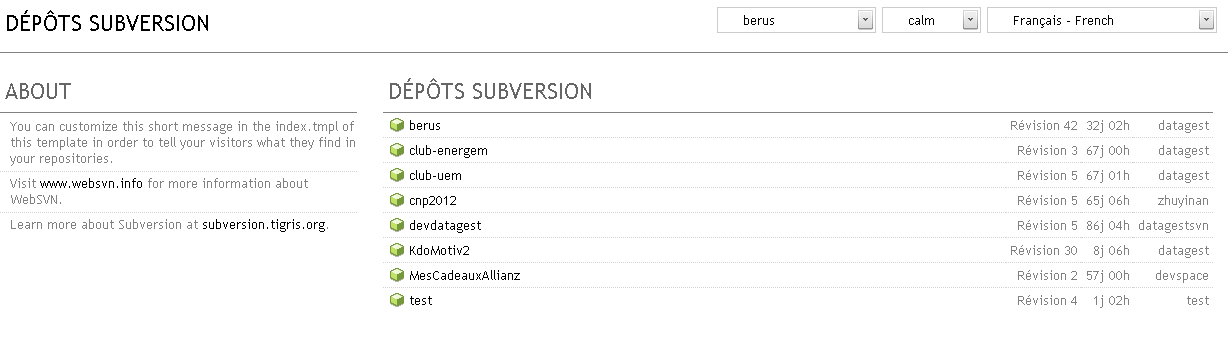
\includegraphics[width=15cm]{body/images/websvn.png}
\caption{Interface WEBSVN}
\end{figure}


\subsubsection{HOOK}
Un hook (littéralement crochet) permet de lancer un programme personnalisé au moment précis où le programme principal à la tâche de l’exécuter. Dans le cas de svn les hooks sont applicables sur les évènements de contrôle de version( commit , changement de révision, lock). On peut le comparer à la notion de trigger en sql.
On utilise "hook" chaque fois que on fait un commit de local à serveur distant afin de aussi mettre à jour de modification dans le répertoire où le site est situé. C'est très pratique pour le debug.

Ce que on a utilisé dans hook est l'événement \textbf{post-commit} , une notification du succés de la transaction de commit. Généralement utilisé pour envoyer un mail à un administrateur ou synchroniser le site 


\subsection{Création de la documentation du Data-Gest}
\paragraph{}
Avant je suis arrivé, il n'y a rien de documentation de pôle web chez Data-Gest, c'est la raison que je voudrais créer la documentation de noter ce que j'ai fait. Dans variés types des applications de wiki, j'ai choisi dokuwiki comme le wiki de Data-Gest basé sur les raison suivant.
\begin{figure}[hbtp]
\centering

\includegraphics[width=5cm]{body/images/dukowiki.png}
\caption{Dokuwiki}
\end{figure}
\begin{itemize}
\item [-] C'est un moteur de wiki libre sous licence GUN GPL
\item [-] Simple à utiliser et déployer comme il est développé en PHP.
\item [-] Le plus important avantages est que toutes les données sont stockées dans des fichiers texte, et donc aucune base de données n’est nécessaire. C'est très pratique pour la migration.
\end{itemize}

\paragraph{}
J'ai noté tous lès points importants sur le wiki pendant mon travail. Par exemple, comment changer la version de PHP sur serveur distant en utilisant fichier .htaccess. 

En plus j'ai aussi rédigé la documentation sur comment gérer des dépôts SVN sur serveur distant, les informations de serveur local et serveur distant. 

En fait, la documentation est pour des nouveaux employés afin de intégrer rapidement dans équipe de développement â pôle web chez Data-Gest. 

Voici une liste de contenu j'ai créé dans dokuwiki :
\begin{figure}[hbtp]
\centering
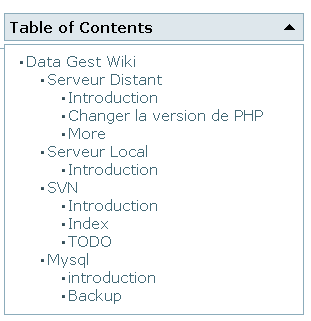
\includegraphics[scale=1]{body/images/dokuwiki-content.png}
\caption{Dokuwiki}
\end{figure}


\newpage
\section[Amélioration KdoMotiv]{Amélioration du framework KdoMotiv}
\subsection*{}
La mission principale pendant mon stage est d'améliorer le framework KdoMotiv médium. En fait KdoMotiv est déjà développé par l'ancien stagiaire. A cause de son niveau de programmation, il ne connaît pas la programmation orienté objet(POO). Par conséquence, tout le framework de KdoMotiv est développé en PHP procédure. Ça cause de problème de maintenance et le debug comme il n'y a pas de documentation, ni de commentaire sur le KdoMotiv, le stagiaire suivant est difficile de maîtriser tout le projet. En plus, après avoir testé la fonctionnement, j'ai trouvé qu'il existe encore beaucoup de erreurs et beaucoup de parties reste à faire.

C'est pourquoi j'ai discuté avec le patron afin de refaire tout de KdoMotiv en PHP objet. Mais comme ça prend du temps et aussi du frais de l'entreprise. Après avoir bien réfléchi les conditions et les situations actuels. Le patron à refusé ma propositions. En plus, je ne peux pas assurer ce que je ferai est stable et mieux que le framework KdoMotv actuel. 

\begin{figure}[hbtp]
\centering

\includegraphics[scale=1]{body/images/kdomotiv.png}
\caption{KdoMotiv Logo}
\end{figure}


Par conséquence, mon tuteur m'a demandé d'améliorer du framework KdoMotiv, y compris le debug et aussi finir des fonctionnalité lesquels on n'a pas encore réalisé, afin de faire un framework plus stable et complet.

Les étapes de conséquences sont comme ci-dessous : 
\begin{enumerate}
\item Debuger tout le site, trouver tous les erreurs dès que possible.
\item Compléter les fonctions qui n'ont pas encore fini.
\item Ajouter nouvelles fonctions et modules sur KdoMotiv.
\item Normaliser les formule afin de adapter à ERP de Data-Gest  
\end{enumerate}

\subsection{Introduction structure de KdoMotiv}
J'ai parlé ici plutôt le KdoMotiv médium. KdoMotiv médium est composé par deux parties principal. Le Back Office et le front office. Ce structure est comme CMS wordpress. Back Office sert à l'administration et la configuration de KdoMotiv. Front Office est l'interface pour les participants de visiter la boutique et les résultats de ses challenges.

On a choisi le projet Beru qui est le projet plus proche et stable en utilisant KdoMotiv, comme le base de nouveau KdoMoitv sur lequel on va faire le nouveaux développement.



\subsection{Debuger KdoMotiv}
La première étape est de debuger tout le site, le Front Office  et aussi Back Office. 
Le debug est composé par :
\begin{itemize}
\item [-] Debug par pages du site. Surtout sur front office.
\item [-] Debug par module du site. Surtout sur back office.
\item [-] Tester la fonctionnalité de site, y compris les étape de commande fonctionne bien, la fonction de mail de confirmation marche bien, etc.
\end{itemize}

J'ai séparé les taches avec mon collègue. il s'est occupé de debuger le Front Office. je me suis occupé de debuger le Back Office.

Les problèmes principales sont toujours des codages de page, lès variable GET et POST ne passe pas a la page suivant etc.


\paragraph{}
Ici j'ai listé les bugs sur front office(FO), les bugs sont testé par chaque page. 

\begin{table}[htbp]
\renewcommand{\tabularxcolumn}[1]{>{\arraybackslash}m{#1}}
\begin{tabularx}{\textwidth}{lX}
\hline 
PAGES
 & BUGS
 \\ 
\hline 
Panier.php
 & header\_information + Problème accents "Qté"
 \\ 
\hline 
Panier.php/livraison
 & Info bulles ne disparaissent pas après écriture dans le champ sépcifié
 \\ 
\hline 
Panier.php/Confirmation
 & Injection sql dans les formulaires suite à injection de caractères bizarres
 \\ 
\hline 
Panier.php/validation
 & Dans le header le solde se traduit avec des points
 \\ 
\hline 
Panier
 & Après une commande, le header affiche le prénom du user au lieu du pseudo, le mot "étoile" n'est plus affiché par rapport à la Validation. Les champs "société" et adresse ne sont pas affichés dans le récapitulatif.
 \\ 
\hline 
Palier
 & Pourquoi une page palier  d'abord alors que les catégories sont déjà listées dans la page boutique.
 \\ 
\hline 
compte.php
 & Relevé d'étoiles ne fonctionne pas.
 \\ 
\hline 
\end{tabularx} 
 \caption{bugs de Front Office}
\end{table}

\paragraph{}
J'ai testé le Back office de KdoMotiv. En plus, j'ai debugé selon la fonctionnalité de backoffice et testé un module par un module. Le page suivant liste tous les bugs pendant mon test. C'est un test totalement et complètement. 

Après le test, j'ai défini le valeur d'importance de chaque bug, et décidé la séquence de résoudre chaque problème. A cause de KdoMotiv est programmé par PHP en procédure dure, en plus , il n'a pas de documentation de KdoMotiv ni de commentaire de code, ça prend du temps de tous les trouver.

\begin{table}[htbp]
\renewcommand{\tabularxcolumn}[1]{>{\arraybackslash}m{#1}}
\begin{tabularx}{\textwidth}{lX}
\hline 
MODULES & BUGS \\ 
\hline 
Tous
 & Change le logo de backoffice. Il faut trouver que si le logo de BO et FO est configuré dans même endoit
 \\ 
\hline 
Menu bar
 & Par très compatible avec chrome, quelque fois on ne peut pas choisir le sous-onglet de menu
 \\ 
\hline 
Participants
 & Il faut utiliser jqgrid pour la gestion. Il faut ajouter un lien pour accéder à la détail des information de chaque participant. Aussi changer le titre
 \\ 
\hline 
• & Pour modifier le détail de participant, je ne peux pas tester, il depend un pear extension qui n'est pas installé sur serveur dev
 \\ 
\hline 
Commandes
 & Change le titre. Pour la liste, soit on ajouter le lien d'accéder pour voir le détail de commande, soit on fait un sous jqgrid table pour voir le détail de commande.
 \\ 
\hline 
Cadeaux
 & Dans le colonne  "univers", le type "tous" c'est pas le valeur par défaut pour le recherche. Mais j'ai déjà tester tous le méthode, ce ne marche pas pour le mettre à le premier positon pour le recherche.
 \\ 
\hline 
CMS
 & Contenu de la page résultat -\textgreater je ne sais pas il sert à quoi
 \\ 
\hline 
• & Info popup lightbox -\textgreater Il faut trouver à quoi il  sert 
 \\ 
\hline 
Modules
 & Pour les bouton "supprimer" "modifier" "nouveau", tous ne fonctionne pas.
 \\ 
\hline 
• & New-\textgreater ne peut pas tester à cause de problème de "extension"  n'est pas installer sur serveur dev
 \\ 
\hline 
• & Quiz-\textgreater Un Waring dans entête.  (Quand il y des quiz dans BDD, le warning disparu)  
 \\ 
\hline 
• & Faq-\textgreater Caractère spécieux dans titre de FAQ, dans le contenu , tous c'est bon.   
 \\ 
\hline 
Données
 & Visite du site-\textgreater Ne pouvez pas exporter
 \\ 
\hline 
• & Export des bonus-\textgreater Même problème
 \\ 
\hline 
• & Export tax-\textgreater Pas bonne requête, unknown colonne
 \\ 
\hline 
• & Export des quiz -\textgreater warning dans la tête, si la liste de quiz est vide
 \\ 
\hline 
Configuration
 & Connexion-\textgreater même si on change le base dans BO, il sert à rien
 \\ 
\hline 
• & Logo client -\textgreater sert à rien, rien changer ni dans BO, ni dans FO
 \\ 
\hline 
• & Participant FO-\textgreater fonctionne pas du tous
 \\ 
\hline 
\end{tabularx} 
 \caption{bugs de Back Office}
\end{table}  


\newpage

\subsection{Amélioration du interface graphique de Back Office}
Comme j'ai déjà raconté avant, il y a des problèmes de compatibilités avec la navigation bar dans Back Office. En plus, il y a aussi quelque partie n'affiche pas bon. C'est pourquoi je vais changer toute la intégration HTML de back office.

Dans projet de KdoMotiv, j'ai choisi Twitter Bootstrap comme le framework de intégration HTML. En fait, Twitter Bootstrap est une collection de outils gratuits utilisé pour la création des sites et aussi applications web. Il contient tous les designs basé sur HTML et CSS pour typography, formulaire, bouton, navigation et des autre interface composants, aussi bien que Javascript extensions.

\subsubsection{Changer la navigation bar}
L'ancienne navigation bar est comme la figure cinéma ci-dessous. Il y a non seulement du problème de compatibilité avec différent navigateur, mais aussi pas très claire avec la séparation de fonctionnalité.
\begin{figure}[hbtp]
\centering
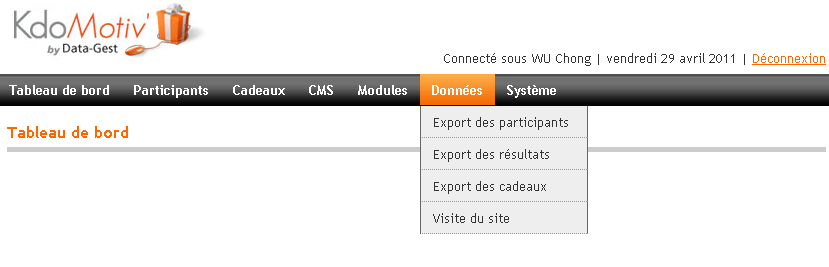
\includegraphics[width=15cm]{body/images/navbar-old.png}
\caption{Ancienne navigation bar}
\end{figure}

Par exemple, on peut trouver tous lès fonctionnalité d'exporter données dans onglet données, mais les fonctionnalité d'importer données sont dans onglet système. Ce n'est pas logique et pratique pour les utilisateur d'administrer.



 \begin{figure}[hbtp]
\centering
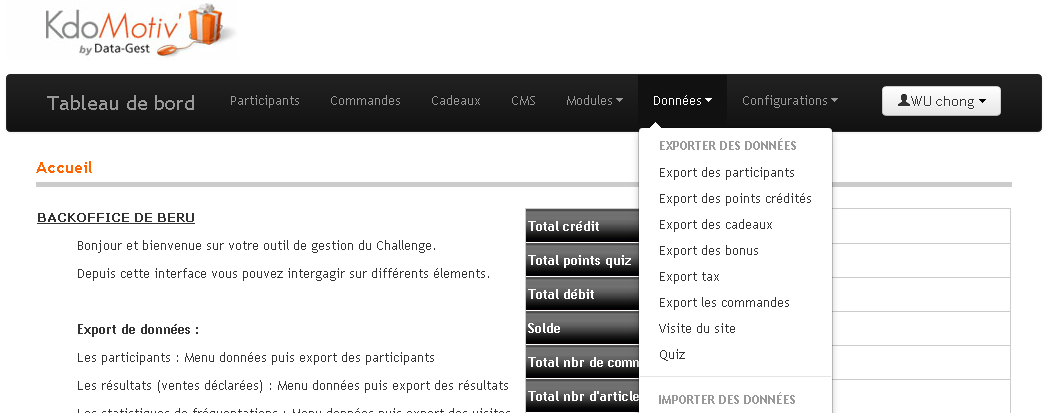
\includegraphics[width=15cm]{body/images/navbar-new.png}
\caption{Nouvelle navigation bar}
\end{figure}

Par contre, dans le framework de Twitter Bootstrap, il y a une navigation bar pré-définit qui est compatible avec tous les navigateur plus proche lesquels soutiennent HTML5 et CSS3.

Dans la nouvelle navigation bar, j'ai intégré tous les informations de connexions dans navigation bar, et aussi séparation les fonctionnalité sous propre onglet, comme les fonctionnalités des données dans la figure ci-dissous. 

 \begin{figure}[hbtp]
\centering
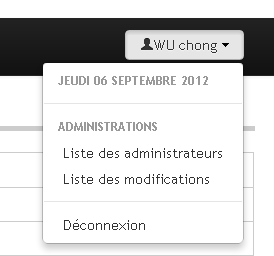
\includegraphics[width=5cm]{body/images/info-connexion.png}
\caption{Nouvelle navigation bar}
\end{figure}

En plus, j'ai aussi ajouter une petite fonction de fixer la navigation bar en haut quand le navigateur détecte l'événement de scroll. Cette fonction est pratique quand le contenu de page est très long mais on va aussi utiliser la navigation bar.

J'ai aussi changé des autre pages et les met dans le cadre de Twitter Bootstrap. Par exemple, le page de participant, qui sert à la gestion des participant de challenge, le page de la configuration , tous les "alert-box" sont utilisés Bootstrap.
\begin{figure}
  \centering
  \subfigure[Ancien sidebar]{\label{fig:Ancien side bar}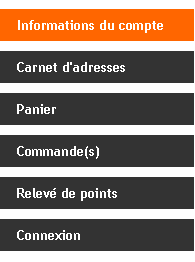
\includegraphics[width=0.2\textwidth]{body/images/sidebar-old.png}}                
  \subfigure[Nouveau sidebar]{\label{fig:Nouveau side bar}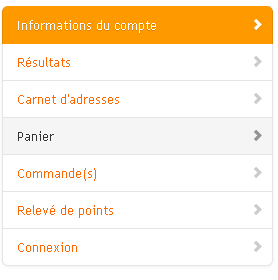
\includegraphics[width=0.2\textwidth]{body/images/sidebar-new.png}}
  \caption{Amélioration du sidebar}
  %\label{fig:Amélioration du sidebar}
\end{figure}



\subsection{Amélioration des formulaires}

\subsubsection{PEAR Qucik Form}
Il y a beaucoup de cas on doit utiliser formulaire dans Back office.
Par exemple, quand on gère  des participant, il faut toujours utiliser les formulaire de modifier les informations de participant, le formulaire de changer le carnet d'adresse de participant, aussi les résultats de participant. 

Mais dans le ancien KdoMotiv, comme il est programmé par PHP en procédure, ce n'est pas facile de tous lès contrôler, il y a environ vingtaine formulaires, les fonctionnalité sont presque la même, mais il faut toujours répéter de refait le formulaire.

Dans ce cas, j'ai introduit une extension dans PERA \footnote{PHP Extension and Application Repository} qui s'appelle PHP quick form. C'est une extension de développer formulaire rapidement. Tous les formulaire sont généré automatiquement selon les variables lesquelles j'ai donné dans un tableau. 

\begin{figure}[hbtp]
\centering

\includegraphics[width=3cm]{body/images/pear_logo.png}
\caption{Logo PEAR}
\end{figure}


Afin de appliquer le Quick Form, il faut installer PEAR sur le serveur. J'ai demandé a l'administrateur d'OVH de me donne le droit lancer commande "PEAR" sur le serveur distant. Ensuite, j'ai juste mis à jour de PEAR et installé  les modules dépendants. 

\begin{figure}[hbtp]
\centering
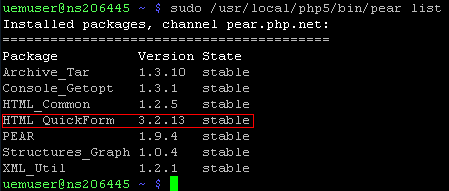
\includegraphics[width=10cm]{body/images/pear_quickform.png}
\caption{PEAR Quick Form}
\end{figure}

Après j'ai réussi d'installer Quick-Form, on peut le trouver dans la liste de PEAR. L'utilisation du Quick Form est facile. (Quick Form utilise la programmation orienté objet) Comme les étapes suivants.
\begin{enumerate}
\item Créer une classe de formulaire.
\item Ajouter les éléments de formulaire.
\item Ajouter les règles de contraintes de formulaire.
\item Générer le formulaire automatiquement. 
\end{enumerate}

J'ai remplacé tous des formulaire traditionnel par Quick Form dans KdoMotiv Back Office.

\subsubsection{Contrôler le longueur du champs}
Quand on passe tous les commande à ERP, il faut contrôler le longueur de chaque champs comme il y a des contraintes de longueur sur les champs de matricule, adresse, adresse complet , dans l'application de ERP(Navision) et aussi l'application d'expédition(La Poste)

Par conséquence, il faut les tous contrôler afin de ne pas poser des erreurs quand on injecte des données dans la base de Data-Gest.

\subsection{Gestion des tableaux avec jqGrid}
Dans le back office de KdoMotiv, on doit utiliser beaucoup de tableaux. Par exemple, la liste de tableau de participant, la liste de tableau de cadeaux, la liste de tableau de commandes passés, etc. Il y a souvent des opérations de modifier, insérer, supprimer, rechercher sur les données dans le tableau.

Mon tuteur de m'a introduit le jqGrid, et demandé de remplacer tous les tableaux par jqGrid ,qui est une libraire utilisée pour la création de tableaux multidimensionnels complexes.

En fait, Data-Gest a déjà acheté la licence de jqGird,  Mais pas encore tous intégré dans le framework de KdoMotiv. 

Le principe de jqGrid est comme ci-dissous:
Une instance d’un jqGrid est un objet javascript avec des propriétés, des évènements et des méthodes. Les propriétés peuvent être de valeur numérique, alphabétique, booléenne, de  tableau ou même d’un autre objet. La convention de base ci-dessous vous permettra de créer la base d’un jqGrid avec les options qu’elle doit contenir par défaut.

\begin{lstlisting}[language= html, numbers=left, numberstyle=\tiny,  frame=shadowbox]
<div id="jqGrid">
      <table id="grid"></table>
      <div id="gridPager"></div>
</div>
\end{lstlisting}

Quand on crée un instance et attribue tous variables nécessaire, le tableau va générer automatiquement.

Mais quand on va créer une tableau plus avancé, par exemple , un sous-tableau dans tableau mère, ou en utilisant AJAX pendant le recherche ,etc. Il faut lire la documentation de jqgrid.

Ci-dessous un exemple de liste de tableau lequel j'ai réalisé par jqGrid.
\begin{figure}[hbtp]
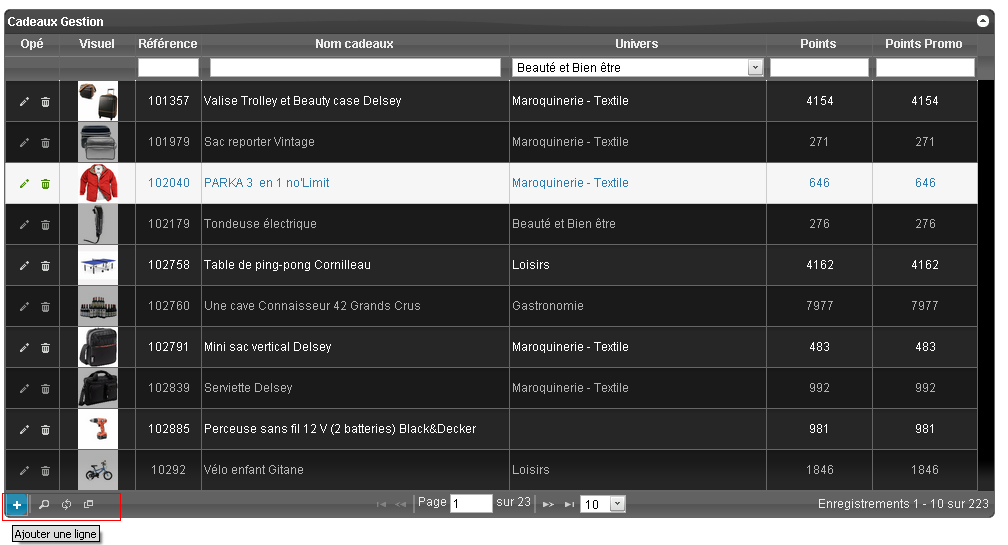
\includegraphics[width=16cm]{body/images/cadeau-new.png}
\caption{Liste de cadeau par jgGrid}
\end{figure}

\begin{figure}[hbtp]
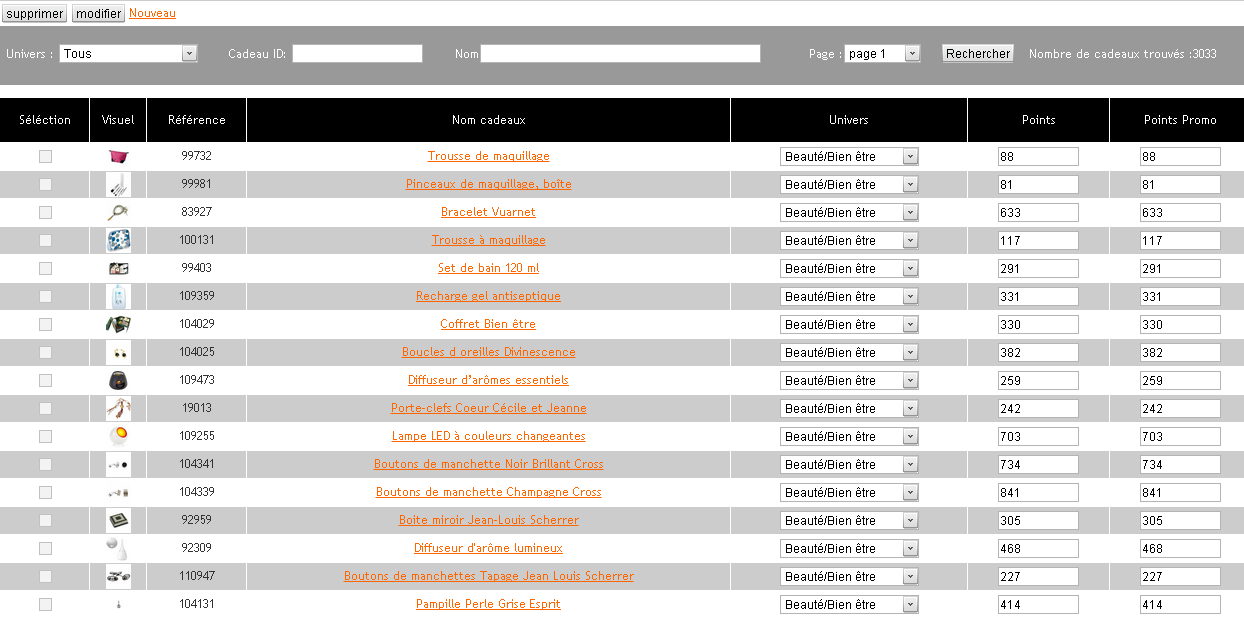
\includegraphics[width=16cm]{body/images/cadeau-old.png}
\caption{Ancien liste de cadeau par jgGrid}
\end{figure}

Par rapport à ancienne version de tableau, tous les opérations de données sont intégrés dans le tableau. L'opération de recherche est plus avancé que l'ancien tableau. En plus, il y a une fonction d'exporter des résultats de tableau en EXCEL ou PDF. Et aussi une mieux pagination.

Comme c'est un logiciel avec licence privée, sauf que la documentation officiel de jqGrid, il n'y a pas de autre solution si j'ai eu les problèmes. Il y a un problème je n'ai pas encore résolu : 
Dans la requête de SQL, il n'accepte pas les variable de GET et POST de PHP. 

\subsection{Mettre des module modulable}
Dans le back office, il faut ajouter les fonctions de mettre des module modulabe. Par exemple, si l'administrateur de site va désactiver le module de résultat afin de ne pas affiche des résultats de participant sur front office, il n'a pas besoin de demander à pôle web de modifier les code, par contre, c'est juste un bouton de contrôler. 

Afin de réaliser cette fonction, il faut créer une table dans le base qui sert à sauvegarder tous les paramètres de configurations.  

Les tables de configurations sont crées selon la différente fonctionnalité. 
\begin{figure}[hbtp]
\centering
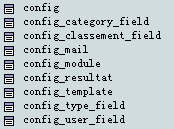
\includegraphics[width=4cm]{body/images/config.png}
\caption{Configuration des tables}
\end{figure}



 
	
\newpage
\section{Projets Réalisé}
\subsection{Introduction}
Pendent mon stage,  j'ai réalisé plusieurs projet simultanément quand je me suis occupé de la améliorer de framework KdoMotiv.

Voici une liste de projet j'ai réalisé pendant 6 mois. (Par ordre de date)

\begin{table}[htbp]
\centering
\renewcommand{\tabularxcolumn}[1]{>{\arraybackslash}m{#1}}
\begin{tabularx}{\textwidth}{lXl}
  \toprule
  Projet & Description  & Durée  \\
  \midrule
	 Beru (BorgWarner BERU )& Challenge de beru basé sur KdoMotiv & 1 mois \\ 	 
	 \hline	 
	 CNP 2012 & Challenge de CNP 2012 sur mesure & 3 semaines \\ 	 
	 \hline
	 Air France & Challeng'air acceptation & 1 mois \\ 
	 \hline
	 Mail listing & Mail de relancer et challenge chaque mois d'Air France & 2 fois chaque mois\\
	 \hline
	 Comité Entreprise & Challenge basé sur KdoMotiv version 2 & Pas encore fini \\
  \bottomrule
\end{tabularx}
 \caption{Liste de projet réalisé }
\end{table}

\subsection{Projet Beru}

\subsubsection{Description}
Le projet beru est le premier grand projet j'ai réalisé pendant mon stage. Il est basé sur l'ancienne version de KdoMotiv. Mais il y a un peu de différence.

\begin{figure}[hbtp]
\centering

\includegraphics[width=10cm]{body/images/projet-beru.png}
\caption{Projet beru logo}
\end{figure}

\begin{itemize}
\item [-] Les participants ne sont pas individuel, c'est les garages de Beru. Mais quand le commande est passé, il est passé par l'employé de chaque garage. c'est différent de principe de KdoMotiv.
\item [-] Compte tenu de la nouvelle législation concernant les gratifications versées par les entreprises aux salariés d'une entreprise tierce, les gagnants devront déclarer aux administrations fiscales les gains perçus. 
\item [-] A cause de problème des informations fiscales, chaque participant ne peut commander qu'un article chaque fois. s'il va commander plusieurs articles, il faut passer plusieurs commandes.
\item [-] Comme les participant sont garages de beru, mais l'adresse de livraison sont selon les employés dans le garage, il faut modifier la structure de KdoMotiv 
\end{itemize}

\subsubsection{Intégration du HTML}
Le projet beru est une copie de projet Club-UEM. Tous les modifications sont basé sur ce projet. Après on a reçu le graphisme de projet beru, j'ai fait la intégration du HTML(PSD\footnote{Fichier de Photoshop} à html). C'est une  méthode que j'ai appris dans le UV de LO18 à UTC.  

Pendant l'intégration , j'ai trouvé que les travaux principal sont le changement de LOGO et bandeau d'entreprise sur KdoMotiv. Par conséquence, j'ai proposé une solution de mettre le logo et bandeau d'entreprise gérable dans Back Office. En plus, j'ai pré-définit trois thèmes graphiques, afin de déployer un projet plus rapide prochainement.

\begin{figure}[hbtp]
\centering
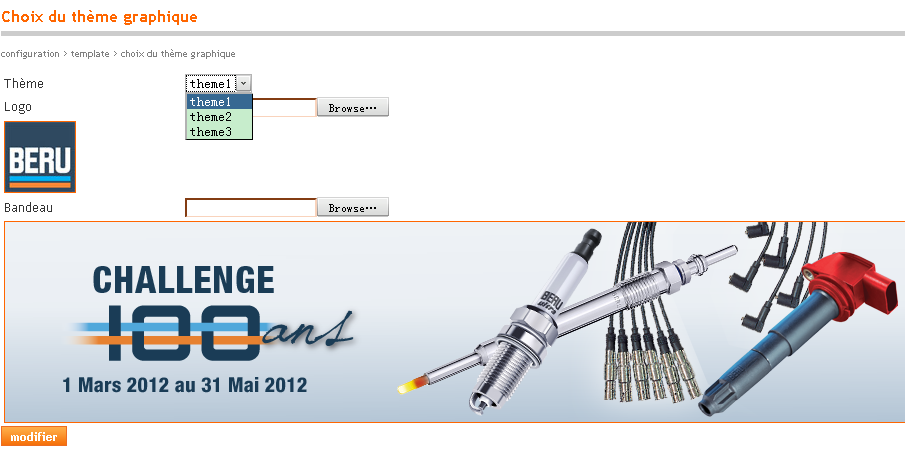
\includegraphics[width=16cm]{body/images/template-theme.png}
\caption{Choix du thème graphique}
\end{figure}
 


\subsection{Projet CNP 2012}
CNP est un client depuis 2011. Le nouveau challenge de 2012 est un projet sur mesure. La structure de site et base de donnée sont totalement différent de la structure de KdoMotiv.

\begin{figure}[hbtp]
\centering

\includegraphics[width=10cm]{body/images/cnp-2012.png}
\caption{Challenge CNP 2012}
\end{figure}

En fait, on a dupliqué le projet de CNP 2011 basé sur lequel on a développé le projet CNP 2012.

\subsubsection{Difficultés} 
Le plus difficile de nouveau projet est de la partie intégration du HTML. Le client nous a offre le fichier de PSD de graphisme, il y a trop de images qui doivent couper, et aussi des décalages de images. Finalement, la partie d'intégration HTML était sous-traité. 

La fonctionnalité du site CNP est différent de KdoMotiv. Il faut refaire noyau du site pour adapter le besoin de client. 



\subsection{Projet Challeng'air}

\subsubsection{Acceptation}
Challeng'air est un projet de Air France.  Il est composé par deux parties, l'inscription et l'acceptation. Je m'occupe de la partie acceptation.
Quand les participant sont passé l'étape d'inscription, et ont validé ses informations personnel, ils peuvent accéder à la page d'acceptation. 
\begin{figure}[hbtp]
\caption{Challeng'air Logo}
\centering

\includegraphics[width=7cm]{body/images/challengair.png}
\end{figure}

En fait, l'acceptation est juste un formulaire à remplir par les participants.  Mais le formulaire est différent entre différents participants selon ses résultats. Soit le participant gagne une carte de cadeau de 30 euro ou 50 euro ,il faut remplir juste des informations de fiscales. Soit le participant gagné un petit cadeau, il faut remplir en plus l'adresse de livraison. 

Afin de réaliser cette fonction, j'ai ajouté la condition de contrôler l'affichage du formulaire d'adresse livraison  selon les cadeaux les participant gagnent. 

C'est aussi nécessaire de contrôler le longueur de champs comme j'ai raconté avant(Bien adapter le ERP de Data-Gest) . Dans ce projet, j'ai utilisé une extension de jqurey(vanadiumjs) afin de limiter des caractères entré de côté client. Au cas où le client désactive javascript , j'ai aussi fait une validation de formulaire de côté serveur en PHP.

\subsubsection{Mailing Liste}
Il y a aussi une mailing list de projet de \textbf{challeng'air}. Comme le besoin de client, il faut envoyer aux participant un  mail de challenge ou un mail de relancer chaque mois. 

La première fois quand j'ai créé un mail de challenge, je l'ai traité plutôt comme une page , j'ai séparé le CSS et  HTML dans différent répertoire. En plus, j'ai utilisé balisé \textbf{div}. Par conséquence, ça cause du problème de l'affichage dans boit de mail.

En fait, ce genre de mail doit être tous ingéré dans une balise \textbf{table}, inclure des codes CSS. Comme la structure ci-dessous:
\begin{lstlisting}[language= html, numbers=left, numberstyle=\tiny,  frame=shadowbox]
<table border=1>
	<tr>
      <td style="..">...</td>
    </tr> 
</table>
\end{lstlisting}

Après j'ai fini le template de mail de premier mois, et testé réussi dans boîte mail de Gmail, YAHOO!,Hotmail. C'est plus rapide de déployer des mails les mois suivants. 
   
\subsection{Projet Comité Entreprise}
Projet Comité Entreprise est le dernière projet avant je suis parti. Il est basé sur KdoMotiv version 2. Mais, il n'a pas besoin de page résultats et page carnet d'adresse comme les demandes de client.  

Par conséquence, j'ai ajouté deux fonctions dans back office afin de faire résultats et carnet d'adresse modulable. 

Ce projet n'est pas encore fini quand je suis parti.




